\subsubsection{Esami}

\begin{scenario}{Scenario: La pianificazione di un nuovo esame}
  Ho un esame importante tra qualche mese e ho deciso di usare BrainBox per organizzarmi. Inizialmente ho perso diversi minuti a cercare la sezione giusta: non avrei mai immaginato che la pianificazione si trovasse sotto la voce \textit{«StudyFlow AI»}, un nome che trovo \textbf{poco pertinente e fuorviante}.

  Una volta entrato, clicco sul pulsante \textit{«NEW EXAM»}. Il sistema mi chiede di inserire il nome della materia e la data. Dopo aver salvato, l'esame compare in lista e noto che il sistema mi mostra quanti giorni mancano alla prova. Tuttavia, mi rendo conto che \textbf{la configurazione è solo all'inizio}. Per aggiungere i task di studio, non posso farlo durante la creazione, ma devo cliccare in un riquadro separato accanto alla lista; avrei decisamente preferito inserire queste scadenze \textbf{direttamente nel modulo di configurazione iniziale}, non solo in un secondo momento.

  Il percorso diventa ancora più macchinoso quando scopro di poter collegare del materiale salvato ne \textit{«I Miei Appunti»}: anche in questo caso, il sistema \textbf{non me lo ha proposto durante la creazione dell'esame}, obbligandomi a ulteriori passaggi manuali. La cosa più grave, però, accade quando ho bisogno di fare delle modifiche: mi accorgo che \textbf{non esiste un modo per eliminare, rinominare o cambiare la data} di un esame già creato. Se sbaglio, sono costretto a ricominciare da capo.

  Inoltre, se entro nel dettaglio di un esame, mi imbatto in un
  \textbf{calendario non ancora funzionante}. In ogni caso, trovo poco sensato poter accedere ai miei impegni solo quando mi trovo confinato dentro una specifica
  sezione: avrei preferito avere il mio calendario \textbf{sempre a portata di mano},
  da qualsiasi parte del sito. Infine, noto che il sistema crea
  \textbf{confusione tra gli esami passati e quelli ancora da sostenere}, mostrandomi tutto insieme senza alcuna distinzione.
\end{scenario}

Lo scenario mette in luce una serie di criticità che frammentano l'esperienza dell'utente in più punti: dalla difficoltà iniziale nel trovare la sezione, al flusso di creazione incompleto, fino all'assenza di opzioni di modifica e a un calendario non operativo. Il risultato è un percorso discontinuo, in cui l'utente è costretto a tornare più volte sugli stessi passi per completare un'operazione che dovrebbe essere lineare. Per rispondere a questi problemi,
la riprogettazione ha puntato a consolidare l'intero flusso in un'unica esperienza coerente.

Nella versione riprogettata, la sezione Esami, ex \textit{StudyFlow AI}, permette all'utente di gestire i propri esami universitari in un unico spazio: è possibile creare un esame, collegare a esso i propri file di studio già caricati in \textit{Appunti} e definire un elenco di attività da completare per prepararsi al meglio. Le scadenze degli esami inseriti 
vengono inoltre riportate automaticamente nel calendario della navbar, così l'utente può verificare in qualsiasi momento quanto manca a ciascun appello senza dover accedere alla sezione dedicata.

\paragraph{Design pattern applicati}
\begin{itemize}

\item \textbf{Modal Panel} (Tidwell): Il pattern prevede l'utilizzo di un pannello sovrapposto alla schermata corrente che blocca temporaneamente l'interazione con il resto dell'interfaccia, concentrando l'attenzione dell'utente su una singola azione focalizzata. È particolarmente adatto per richiedere conferma prima di operazioni distruttive e irreversibili, come l'eliminazione di un elemento, poiché impedisce che l'azione venga eseguita per errore o distrazione. Nella versione precedente l'eliminazione di una task mostrava un messaggio dal testo ambiguo e inaspettato, e non era possibile eliminare un esame. Nella versione riprogettata entrambe le operazioni presentano un Modal Panel dedicato che chiede esplicitamente conferma prima di procedere, rendendo l'azione comprensibile e reversibile fino all'ultimo.

  Problemi di usabilità risolti:
  \begin{itemize}
    \item P87 (Eliminando una task compare un avviso dal testo strano): È stato sostituito con un Modal Panel dal testo chiaro e coerente con il contesto.
    \item P91 (Impossibile eliminare un esame, solo crearne di nuovi): È stata aggiunta la possibilità di eliminare un esame tramite un'azione dedicata, con relativo Modal Panel di conferma.
  \end{itemize}

  \begin{figure}[H]
    \centering
    
\includegraphics[width=0.6\textwidth]{figures/fig-riprogettazione-fisica/esami/esami_7.png}
    \caption{}
    \label{fig:esami_7}
  \end{figure}

\item \textbf{Error Messages} (Tidwell): Il pattern prevede di mostrare messaggi di errore direttamente accanto al campo che li ha generati, in modo che l'utente capisca immediatamente cosa non va e come correggerlo. Nel form di inserimento di un nuovo esame mancava qualsiasi controllo sulla data: era possibile inserire una 
data antecedente a quella corrente, generando un esame che non veniva poi visualizzato nella pagina principale senza alcuna spiegazione. Nella versione riprogettata, il tentativo di inserire una data passata genera un messaggio di errore direttamente sotto al campo, impedendo il salvataggio e informando l'utente del vincolo violato.

  Problemi di usabilità risolti:
  \begin{itemize}
    \item P84 (Possibile inserire un esame con data antecedente a quella corrente, che poi non viene visualizzato): Il form ora valida la data e genera un messaggio di errore esplicito sotto al campo se si tenta di inserire una data passata.
  \end{itemize}

  \begin{figure}[H]
    \centering
    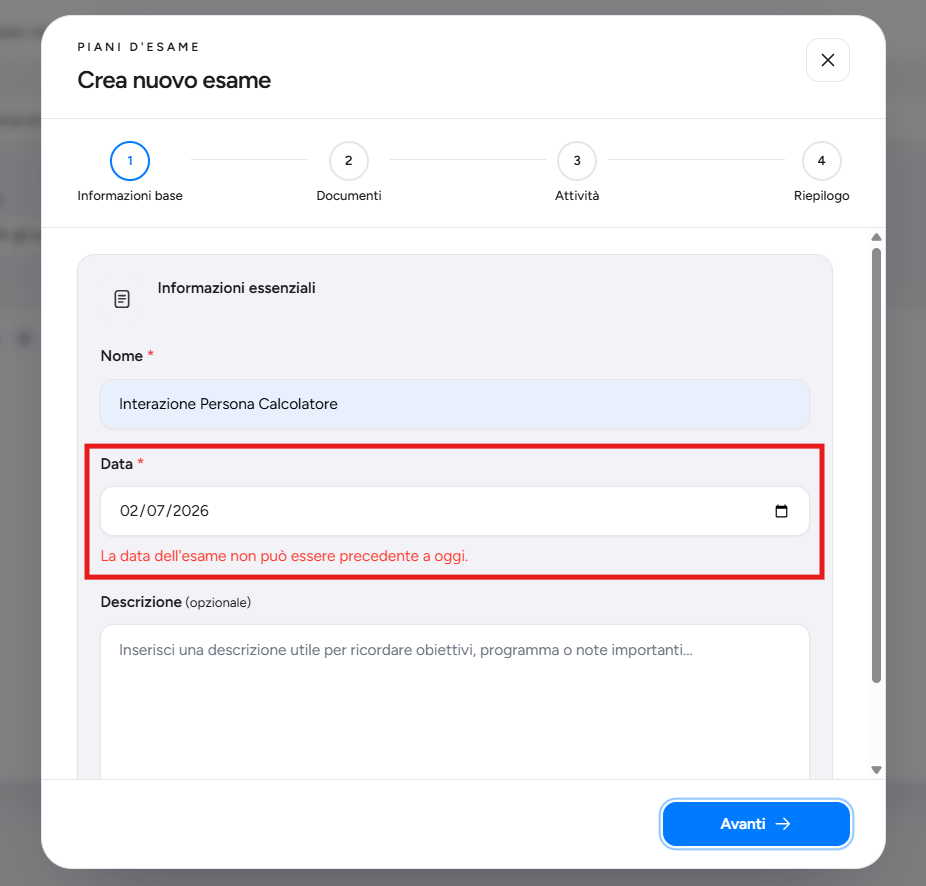
\includegraphics[width=0.6\textwidth]{figures/fig-riprogettazione-fisica/esami/esami_2.png}
    \caption{}
    \label{fig:esami_2}
  \end{figure}

\end{itemize}

\paragraph{Altre modifiche}
È stato adottato un linguaggio coerente con le altre sezioni: la sezione è stata rinominata \textit{Esami} e il pulsante \textit{NEW EXAM} è stato sostituito con \textit{+ Nuovo}, in linea con la convenzione adottata nelle altre sezioni.

Nella visualizzazione dei dettagli di un esame, la gestione del collegamento dei materiali è stata corretta: in precedenza il pulsante \textit{"Aggiungi materiale esistente"} mostrava il messaggio \textit{"Tutti i tuoi documenti sono già stati 
collegati!"} anche quando non era ancora stato caricato nessun file, e il pulsante \textit{"Collega materiali"} compariva privo di funzione attiva. Nella versione riprogettata, quando non sono presenti materiali collegati, compare il messaggio \textit{"Nessun materiale collegato. Usa il pulsante «Aggiungi file» per associare 
appunti esistenti."} e il pulsante risulta correttamente attivo e funzionante. 

\begin{figure}[H]
    \centering
    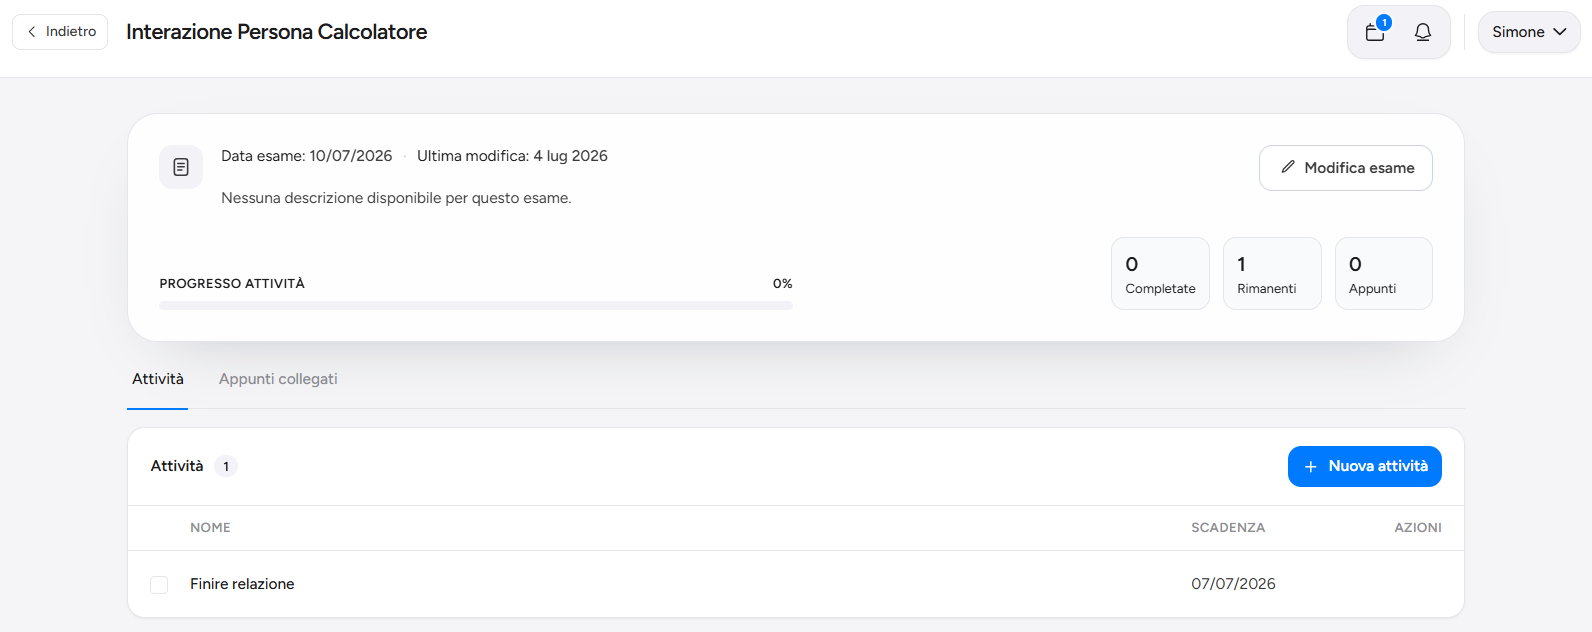
\includegraphics[width=0.8\textwidth]{figures/fig-riprogettazione-fisica/esami/esami_6.png}
    \caption{}
    \label{fig:esami_6}
\end{figure}

Problemi di usabilità risolti:
\begin{itemize}
  \item P46 (Il titolo della pagina non corrisponde al tab selezionato): Il tab \textit{StudyFlow AI} è stato rinominato \textit{Esami} e di conseguenza anche il titolo della pagina.
  \item P47 (Il bottone "NEW EXAM" si trova in una posizione poco funzionale): Il layout è stato allineato a quello delle altre sezioni, con il pulsante \textit{"+ Nuovo"} posizionato in alto a destra accanto alla barra di ricerca e ai filtri.
  \item P48 (Il bottone "NEW EXAM" è scritto in maiuscolo a differenza degli altri): Il pulsante è stato rinominato \textit{+ Nuovo}, in linea con la convenzione adottata nelle altre sezioni.
  \item P49 (La pagina presenta contenuti in inglese): Tutto il testo è stato tradotto in italiano.
  \item P85 (Messaggio "Tutti i tuoi documenti sono già stati collegati!" mostrato anche quando il repository è vuoto): Il messaggio è stato sostituito con un invito contestuale che guida l'utente verso l'azione corretta.
  \item P86 (Il pulsante "Collega materiali" compare senza funzione attiva quando non ci sono materiali): Il pulsante è ora correttamente attivo e funzionante in tutte le condizioni.
\end{itemize}

\paragraph{Implementazioni aggiuntive}
Una delle principali funzionalità aggiunte in questa sezione è quella dei filtri, pensata per aiutare l'utente a orientarsi tra gli esami salvati, risultando particolarmente utile quando questi iniziano ad accumularsi. Si tratta di una funzionalità non direttamente collegata ai problemi emersi durante la valutazione euristica, ma ritenuta fondamentale per migliorare l'esperienza d'uso e per rendere la sezione coerente con quanto già presente in \textit{Appunti} e \textit{Community}.

Il primo è un filtro per stato, che permette di visualizzare tutti gli esami oppure solo quelli preferiti, in corso, completati o scaduti. 
Il secondo è un ordinamento, che consente di riorganizzare la lista per scadenza, nome, progresso o tempo rimanente, in ordine crescente o decrescente.

\begin{figure}[H]
  \centering
  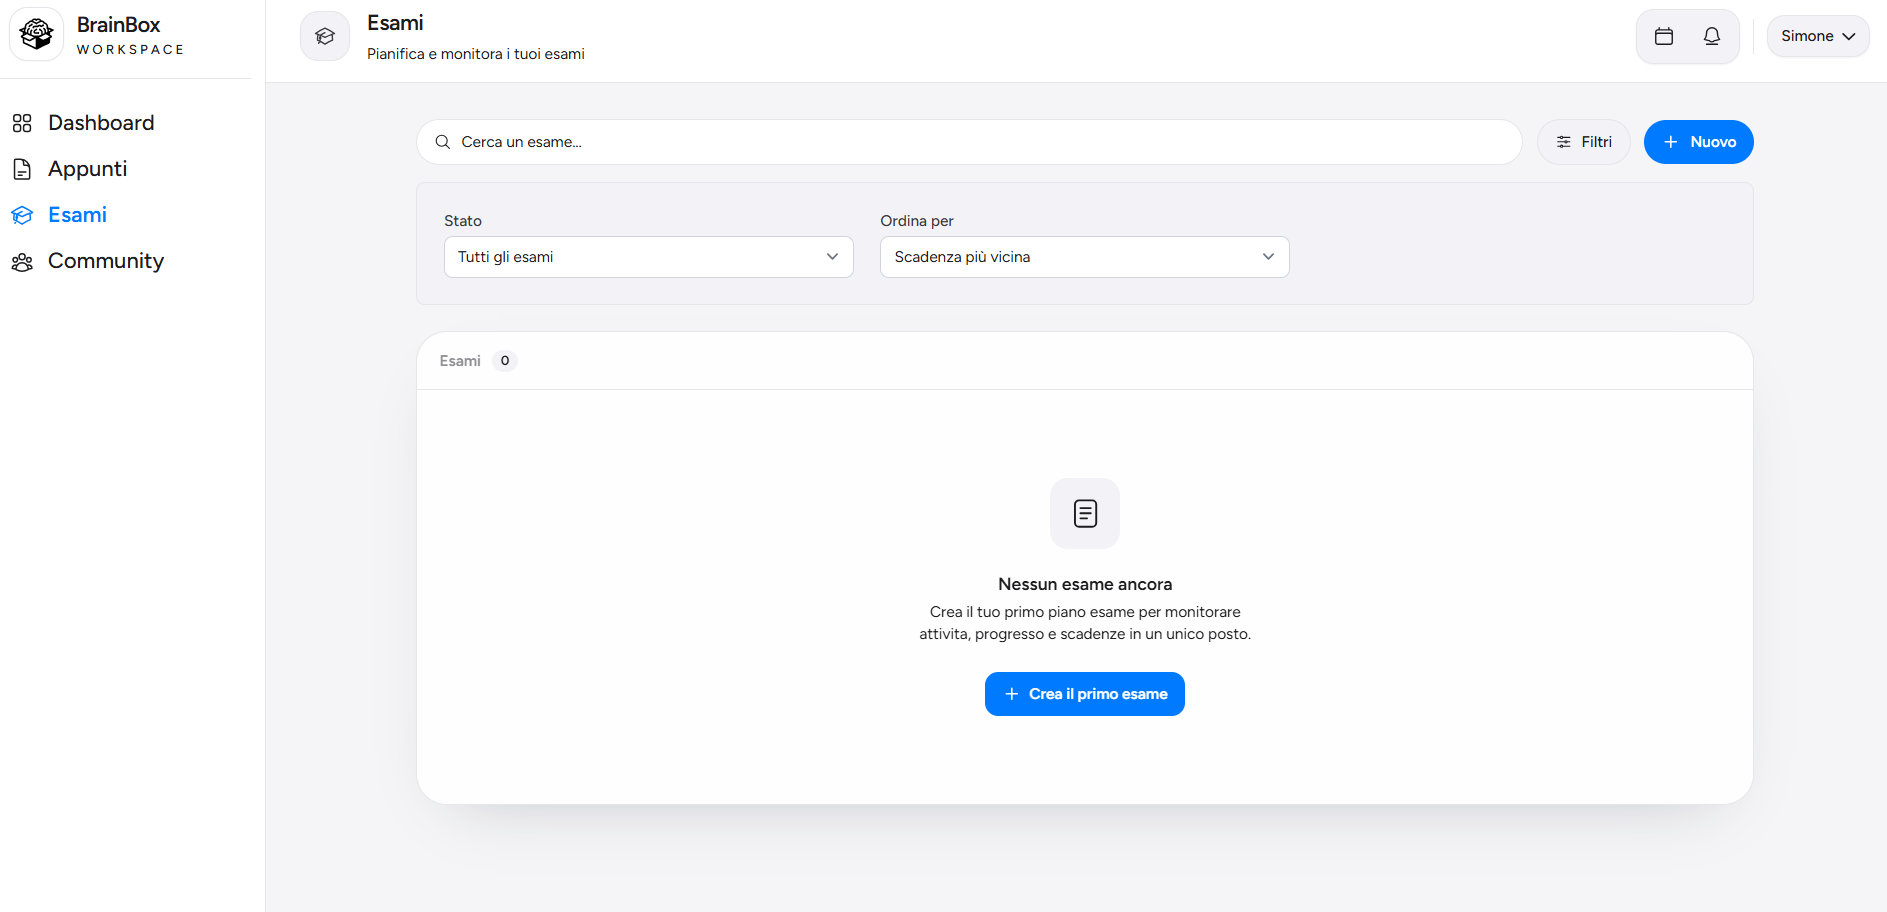
\includegraphics[width=0.8\textwidth]{figures/fig-riprogettazione-fisica/esami/esami_1.png}
  \caption{Pagina iniziale vuota della sezione Esami}
  \label{fig:esami_1}
\end{figure}

\begin{figure}[H]
  \centering
  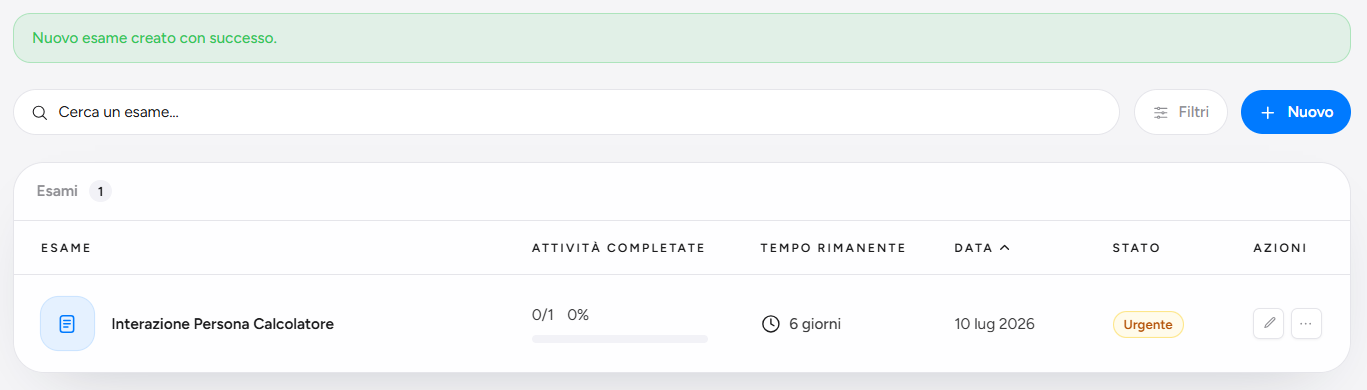
\includegraphics[width=0.8\textwidth]{figures/fig-riprogettazione-fisica/esami/esami_5.png}
  \caption{Pagina iniziale della sezione Esami}
  \label{fig:esami_5}
\end{figure}

Un'ulteriore e fondamentale implementazione ha riguardato l'ottimizzazione del flusso di creazione di un esame. Prima di procedere allo sviluppo dell'interfaccia, si è ritenuto essenziale definire la nuova sequenza operativa attraverso un'analisi dei compiti come riportato in Figura \ref{fig:ta-pianificazione-esame}.

\begin{figure}[H]
  \centering
  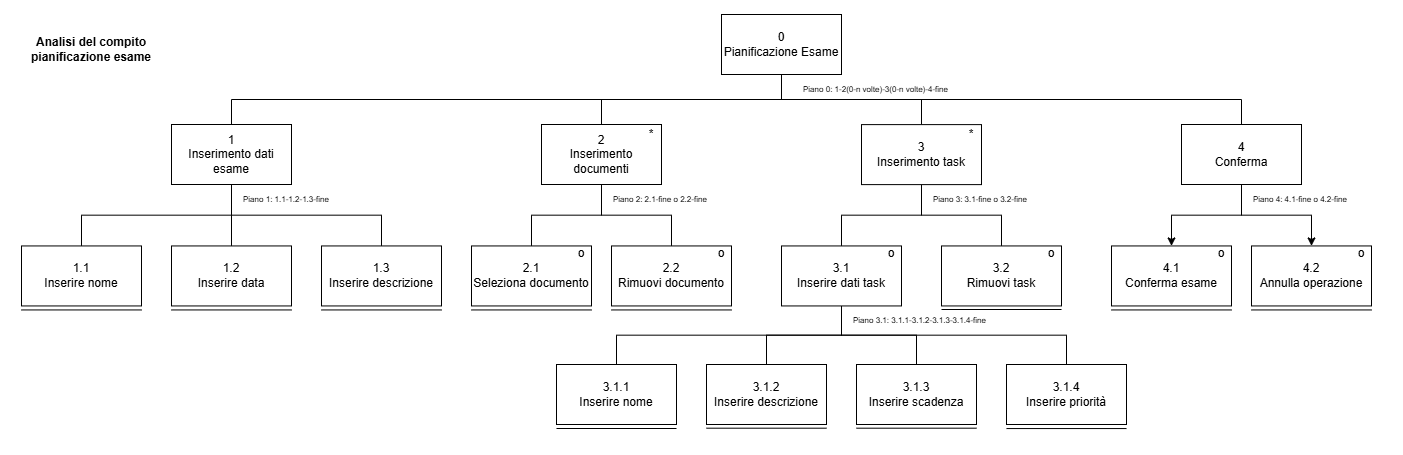
\includegraphics[width=1\textwidth]{figures/fig-riprogettazione-fisica/esami/TA - pianificazione esame.png}
  \caption{Analisi del compito \textit{Pianificazione esame}}
  \label{fig:ta-pianificazione-esame}
\end{figure}

Traducendo concretamente lo schema nell'interfaccia utente, la modale iniziale è stata ampliata introducendo due step aggiuntivi: la definizione delle attività di studio (task) (Figura \ref{fig:esami_3}) e il collegamento dei materiali precedentemente caricati nella sezione \textit{Appunti} (Figura \ref{fig:esami_4}). Questa modifica consente all'utente di configurare un esame completo in un'unica operazione lineare. Al contrario, la versione originale imponeva un processo fortemente frammentato: l'utente era costretto a inserire prima nome e scadenza, per poi doversi spostare in un'area esterna per la creazione dei task e, solo in un secondo momento, accedere al dettaglio dell'esame per collegare i materiali di studio.

\begin{figure}[H]
    \centering
    \begin{subfigure}[b]{0.47\textwidth}
        \centering
        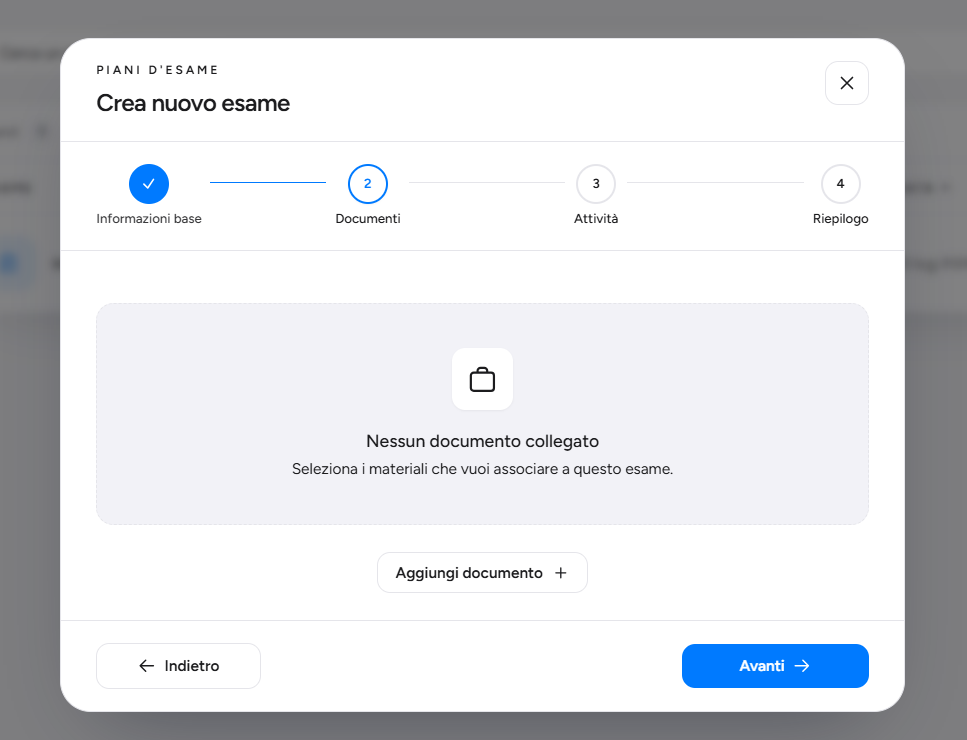
\includegraphics[width=\textwidth]{figures/fig-riprogettazione-fisica/esami/esami_4}
        \caption{Step 2}
        \label{fig:esami_4}
    \end{subfigure}
    \qquad
    \begin{subfigure}[b]{0.47\textwidth}
        \centering
        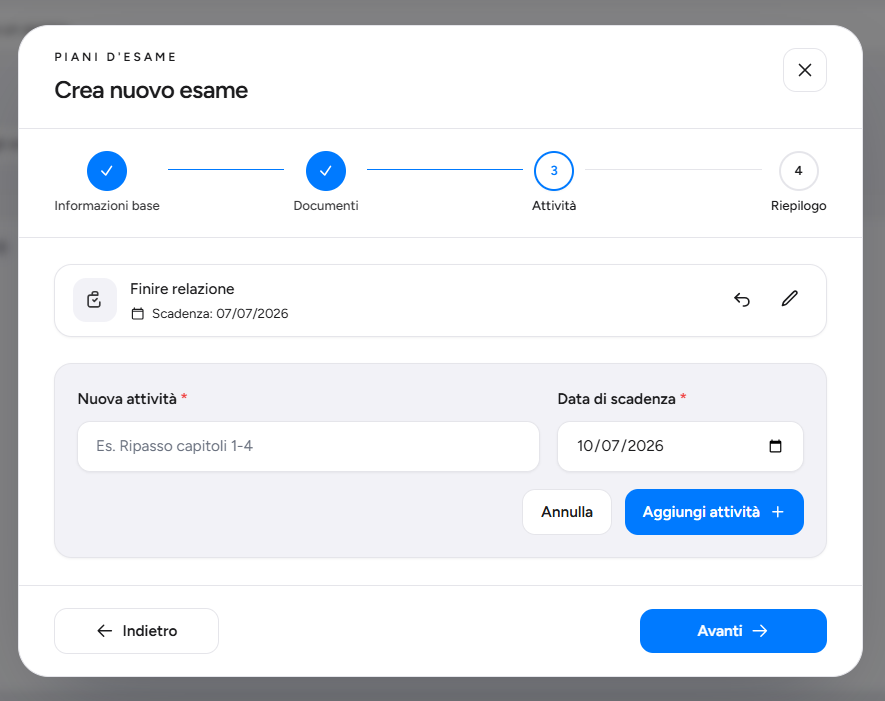
\includegraphics[width=\textwidth]{figures/fig-riprogettazione-fisica/esami/esami_3}
        \caption{Step 3}
        \label{fig:esami_3}
    \end{subfigure}

    \caption{}
    \label{fig:esami_steps}
\end{figure}